\thispagestyle{empty}
\section{Praktische Durchführung}
\subsection{Hardware und Software}


\pagebreak
\subsection{Docker}
Die Docker Container Technologie wurde 2013 als das Open Source Projekt \emph{Docker Engine} eingeführt. Basierend auf Linux Container Konzepten nutzt auch Docker Namespaces und Cgroups zur Isolierung und Limitierung von Containern.  

\subparagraph{Docker Engine}
Docker ist eine client-server Applikation. Der Docker Client kommuniziert mit dem Docker Server oder auch Docker Deamon genannt, der den Großteil der Arbeit übernimmt. Manchmal wird der Docker Deamon auch Docker Engine genannt. Es ist möglich den Docker Deamon und den Docker Client auf demselben Host laufen zu lassen oder den lokalen Docker Client mit dem Docker Deamon auf einem anderen Host zu verbinden. Die Docker-Architektur ist in Abbildung \ref{fig:Docker_Server_Client.PNG} dargestellt \cite{Turnbull2015TheBook}.

\vspace{1em}
\begin{minipage}{\linewidth}
	\centering
	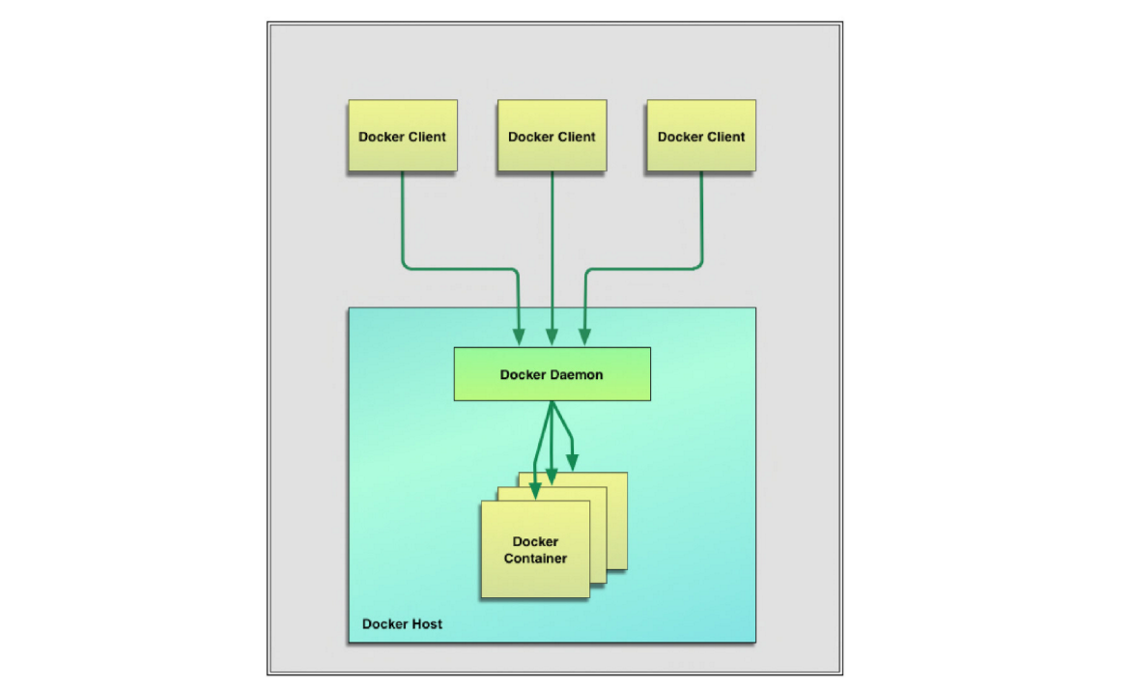
\includegraphics[width=1\linewidth]{pics/Docker_Server_Client.PNG}
	\captionof{figure}[Docker Architektur\cite{Turnbull2015TheBook}]{Docker Architektur}
	\label{fig:Docker_Server_Client.PNG}
\end{minipage}


\subparagraph{Docker Images}
Images sind die Bausteine der Docker Welt. Container werden von Images gestartet. Images sind ein mehrschichtiges Format, die unter Verwendung von Union-Dateisystemen Schritt für Schritt anhand unterschiedlicher Instruktionen erstellt werden. Diese Instruktionen können als Quellcode der Container betrachtet werden. Sie sind einfach verschiebbar und können in Registern verwaltet werden.

\subparagraph{Registries}
Docker speichert die erstellten Images in \emph{Registries}. Es gibt zwei Arten von \emph{Registries}: Öffentliche und private. Docker verwaltet die öffentlichen Images im Docker-Hub\cite{DockerInc.2016DockerHub}. Auf Docker-Hub können eigene Images abgespeichert und geteilt werden. Diese Plattform beinhaltet bereits zehntausende Images, die von anderen Leuten erstellt wurden und für eigene Verwendungen zur Verfügung stehen. Private Images kann man ebenfalls auf \emph{Docker-Hub} abspeichern und niemand außer einem ausgewählten Personenkreis hat Zugriff darauf.

\subparagraph{Docker Containers}
Docker unterstützt beim Erstellen und Ausführen von Containern. Container werden von Images ausgeführt und können einen oder mehrere Prozesse beinhalten. Images können als der Aufbauprozess von Docker gesehen werden und Container als die ausführende Instanz von Docker.

Docker leiht sich das Konzept des Standard Schiff Containers, die für den Transport von Waren eingesetzt werden, als ein Modell für Docker Container, mit dem Unterschied, dass Docker Container keine Waren, sondern Software transportiert. Container können in jeglicher Umgebung ausgeführt werden. Ob auf dem Laptop, nach dem Download von Docker-Hub auf einem Web Server, einem Datenbank- oder auf einem Applikationsserver, die Container werden geladen, wie jeder andere Container auch.

\pagebreak

\subsection{Realisierung}
Das in Kapitel 4 genannte Szenario wird in Teilprobleme zerlegt und schrittweise zusammengefügt. Im ersten Schritt soll gezeigt werden, wie sich der Ressourcenverbrauch eines Containers erhöht und wo eventuelle Grenzen der verwendeten Hardware liegen. Im Linux-File-System ist es möglich, über die PID eines vorhandenen Prozesses die Cgroup herauszufinden, zu der ein Prozess gehört. Zur Erinnerung, jede Cgroup ist für die Ressourcenbegrenzung, Priorisierung, Abrechnung und Kontrolle aller Prozesse zuständig, die unter ihr erstellt wurden. Unter einem Kontrollregister im Linux-Kernel kann die Summe der verwendeten Ressourcen aller unter einer Cgroup laufenden Prozesse zur Laufzeit ausgelesen werden. Die Idee zur Durchführung ist es, einen neuen Docker-Container zu erstellen. In diesem ruft ein Programm in Endlosschleife den malloc() Befehl auf. Dieses Programm wurde in \emph{C} erstellt. Mit Hilfe der Cgroup wird der Speicherverbrauch des Containers überwacht.

\subparagraph{Test01}
Auf Docker-Hub wird ein geeignetes Image ausgesucht und für den Test erweitert. Beim Ausführen des Image wird ein Docker-Container erstellt. Ressourcenlimits können ebenfalls vor dem Starten des Containers eingestellt werden. Für den ersten Start sind allerdings noch keine Begrenzungen des Speichers nötig, da es in erster Linie um die Auswirkung des ausgeführten C-Programms auf die Ressourcenverwaltung im Container geht. Der verwendete C-Code, den der Prozess ausführt, ist in Listing \ref{01mem} zu sehen. Ein erstelltes Skript verwendet die beim Start erzeugte PID, findet die Cgroup in der der Prozess ausgeführt wird und schreibt die ausgelesenen Messdaten in eine Text-Datei. Die Messdaten wie System-Clock-Time in Nanosekunden und Speicherverbrauch in Bytes werden für die Auswertung verwendet.


\vspace{1em}
\lstinputlisting[caption=Einfacher C-Code, label=01mem, basicstyle=\ttfamily\scriptsize]{code/01mem.txt}

\subparagraph{Erwartungshaltung Test 01}
Unter der Annahme, dass das Skript die Messwerte in ungefähr gleichmäßigen Abständen liefert, wird ein linearer Zusammenhang zwischen Zeit und Speicherverbrauch erwartet. Dazu muss die Speicheralokation in jedem Durchlauf stets eine vergleichbare Zeit in Anspruch nehmen. Wenn nicht mehr genug Speicher im System vorhanden ist, wird der OOM-Killer den Prozess beenden.

\vspace{2em}
\begin{minipage}{\linewidth}
	\centering
	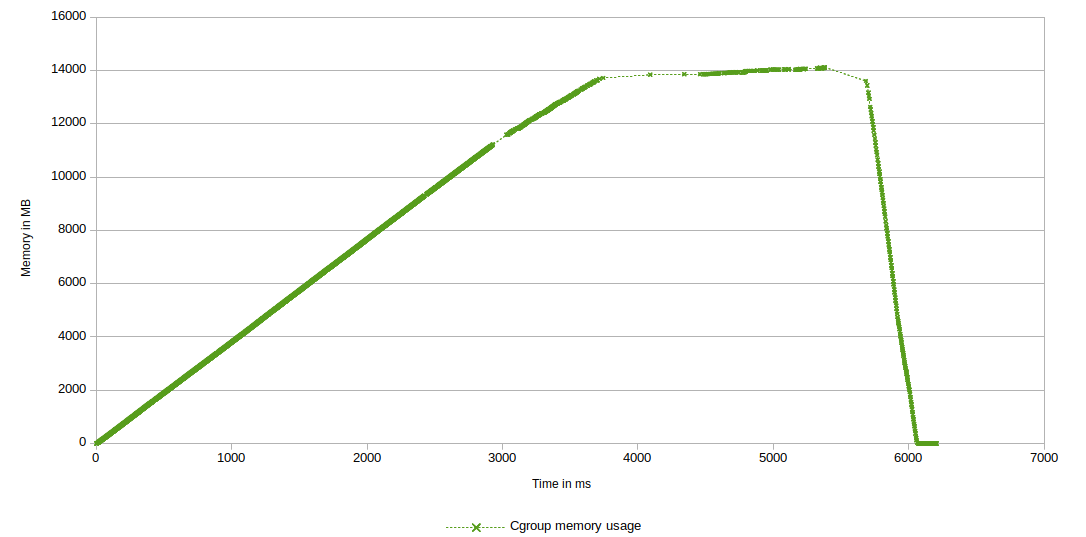
\includegraphics[width=1\linewidth]{pics/001_mem_usage_No_Limit_Cgroup_RDY_FOR_USE.png}
	\captionof{figure}[Speicher Verbrauch Cgroup Ohne Limit]{Memory usage Cgroup no Limit}
	\label{fig:001_mem_usage_No_Limit_Cgroup_RDY_FOR_USE}
\end{minipage}


\subparagraph{Ergebnis Test01}
In Abbildung \ref{fig:001_mem_usage_No_Limit_Cgroup_RDY_FOR_USE} ist wie erwartet ein linearer Zusammenhang erkennbar. Bei ca. 13900MB allokiertem Speicher sättigt die Kurve. An diesem Punkt ist der insgesamt 16GB große Arbeitsspeicher größtenteils ausgeschöpft. Ein paar Megabyte konnten vom Betriebssystem für den dauerhaft nach mehr Speicher verlangendem Prozess gefunden werden. Bei knapp über 14000MB wurde der OOM-Killer eingeschaltet, um wichtigere Prozesse zu schützen und der Container wurde beendet.

\subparagraph{Test02}
Im nächsten Schritt wird der Verlauf einer Cgroup näher betrachtet, bei der ein Speicherlimit festlegt wird, das nicht überschritten werden soll (Hard-Limit). Um dieses Limit zu erstellen, wird das Image entsprechend angepasst und das Speicherlimit auf 8200 Megabyte gesetzt. Das in Listing \ref{01mem} vorgestellte Programm wird wieder ausgeführt.

\subparagraph{Erwartungshaltung Test 02}
Da nun ein Hard-Limit eingerichtet ist, soll die Cgroup mit der gleichen Geschwindigkeit wie in Abbildung \ref{fig:001_mem_usage_No_Limit_Cgroup_RDY_FOR_USE} bis zum gesetzten Limit ansteigen und dieses nicht überschreiten. 

\vspace{1em}
\begin{minipage}{\linewidth}
	\centering
	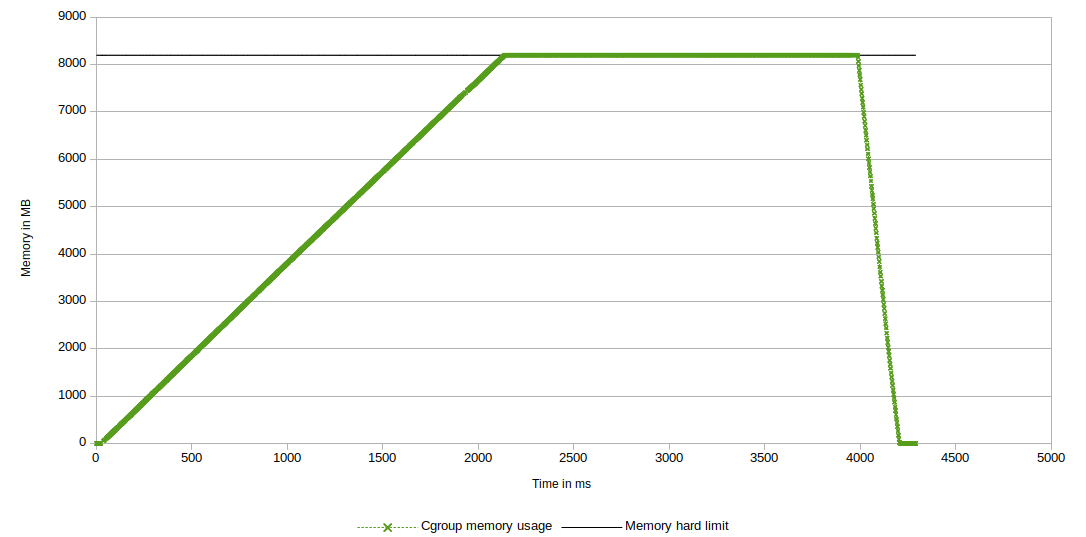
\includegraphics[width=1\linewidth]{pics/002_mem_usage_8200mb_limit_Cgroup_RDY_FOR_USE.png}
	\captionof{figure}[Speicher Verbrauch Cgroup 8200MB Limit]{Memory usage Cgroup 8200MB Limit}
	\label{fig:002_mem_usage_8200mb_limit_Cgroup_RDY_FOR_USE}
\end{minipage}

\subparagraph{Ergebnis Test02}
Mit einer Allokationsrate von ca. 4000MB/S ändert sich die Speicherzugriffsrate nicht. Das Limit von 8200MB wurde erfolgreich eingehalten und der Prozess später vom Betriebssystem beendet.

In Abbildung \ref{fig:001_mem_usage_No_Limit_Cgroup_RDY_FOR_USE}, \ref{fig:002_mem_usage_8200mb_limit_Cgroup_RDY_FOR_USE} tritt eine Sättigung der Speicherallokation ein. Es stellt sich auch die Frage, warum das Programm zu einem späteren Zeitpunkt vom OOM-Killer beendet wird. Das legt den Schluss nahe, dass das Programm weiterhin Speicher vom Betriebssystem erhält, die Cgroup jedoch nicht in der Lage ist, dies zu erfassen. 

Betrachtet man die Cgroup wie eine Box, ist eine mögliche Erklärung für das oben gezeigte Verhalten herleitbar. Die Größe der Box wird bei der Erstellung des Containers festgelegt. In Abbildung \ref{fig:002_mem_usage_8200mb_limit_Cgroup_RDY_FOR_USE} waren es 8200MB. Der Füllstand der Box setzt sich aus den verwendeten Ressourcen aller in der Box ausgeführten Prozesse zusammen. Wenn ein Prozess wie in Abbildung \ref{fig:002_mem_usage_8200mb_limit_Cgroup_RDY_FOR_USE} die komplette Box ausfüllt und weiter darüber hinaus ragen würde, wäre die Box nur in der Lage den Füllstand bis zu Ihrer Maximalgröße von 8200 MB widerzuspiegeln. Der überlaufende Teil des Prozesses kann von der Cgroup nicht erkannt werden.

\subparagraph{Test03}
Nach oben genannter Vermutung liegt es nun nahe, den Speicherverbrauch des Prozesses genauer zu untersuchen. Das Testskript wird erweitert, um die vom Prozess verwendete Anzahl der Memory-Pages auszugeben. Die Anzahl an benötigten Memory-Pages in einem laufenden Prozess, kann ebenfalls im Linux-Kernel ausgelesen werden. Eine Memory-Page ist 4KB groß und ergibt multipliziert mit der verwendeten Anzahl an Memory-Pages die Speichergröße.

\subparagraph{Erwartungshaltung Test 03}
Wenn die Memory-Page Größe multipliziert mit der Anzahl an verwendeten Memory-Pages genau dem entspricht, was die Cgroup an Speicherallokation ausgibt, sollten beide Graphen bis zum Erreichen des Limits deckungsgleich sein.

\vspace{1em}
\begin{minipage}{\linewidth}
	\centering
	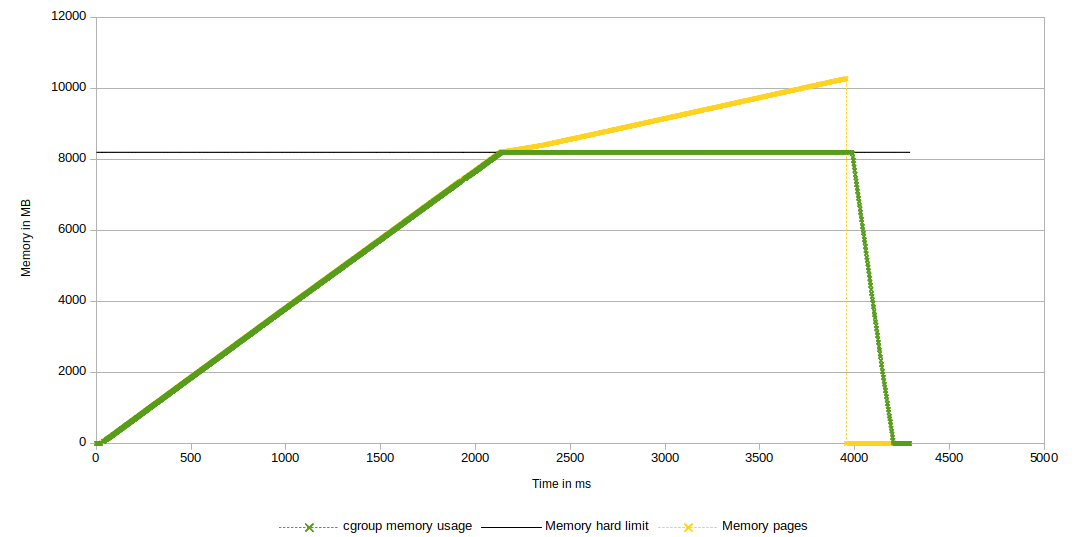
\includegraphics[width=1\linewidth]{pics/003_mem_usage_8200mb_limit_Cgroup_Pages_RDY_FOR_USE.png}
	\captionof{figure}[ Endlosschleife Malloc]{Memory usage Cgroup Memory pages 8200MB Limit Endlosschleife Malloc}
	\label{fig:003_mem_usage_8200mb_limit_Cgroup_Pages_RDY_FOR_USE}
\end{minipage}

\subparagraph{Ergebnis Test03}
Deutlich zu erkennen sind die exakt aufeinanderliegenden Messwerte der Cgroup und der Memory Pages. Ab 8200MB Überschreiten die allokierten Memory Pages bis ca. 10200MB das Limit. Erkennbar ist auch die geringere Allokationsrate die nach dem Überlauf auf 2000MB/s fällt. Komplett ignoriert wurde das Limit allerdings nicht. Verglichen mit Abbildung \ref{fig:001_mem_usage_No_Limit_Cgroup_RDY_FOR_USE} war noch genügend Speicher im System vorhanden. Somit stellen sich folgende Fragen:

Wieso wurde der Prozess dann überhaupt schon beendet, 

warum konnte er über das Limit hinaus allokieren, 

wie verhält sich ein Container, wenn er nur ein wenig über das Limit geht,

wie wirkt sich das auf andere Container im System aus?

Eine mögliche Antwort ist das sogenannte \emph{Paging}. Beim Paging werden allokierte, aber aktuell nicht verwendete Memory Pages vom Arbeitsspeicher auf den Massenspeicher geladen. In Abbildung \ref{fig:003_mem_usage_8200mb_limit_Cgroup_Pages_RDY_FOR_USE} ist nach 8200MB die Trennung zwischen der gelben Linie \emph{Memory pages} und der grünen Linie\emph{Cgroup memory Usage} zu erkennen. Zu diesem Zeitpunkt hat das Betriebssystem mit dem Paging begonnen und lädt von dem Prozess allokierte Pages in den Massenspeicher. Die tatsächliche Menge an Arbeitsspeicher, der von der Cgroup auf der Hardware allokiert ist, bleibt gleich. Die gelbe Linie zeigt die Summe aller vom Prozess allokierten Memory Pages, folglich auch den auf den Massenspeicher ausgelagerten Anteil. Die Steigung der gelben Linie ist durch die Erhöhten Anforderungen an das I/O System, was das Paging zu verantworten hat, zu erklären. Deshalb verringert sich die Allokationsrate beim überschreiten des Limits. Der Überlauf von ca. 2GB stimmt mit dem 2GB Paging-Limit überein.

\subparagraph{Test03,5}
zur Abklärung und Überprüfung des Paging-Limits, empfiehlt sich den Test aus Abbildung \ref{fig:010_mem_usage_8200mb_limit_Container03_undContainer04_RDY_FOR_USE_Focu} mit Erweiterung von Memory Pages zu widerholen.

\subparagraph{Erwartungshaltung Test03,5}
Es wurden ca. 14000MB beim ersten Testdurchlauf allokiert. Mit dem zusätzlichen Paging Limit von 2GB sind die Memory Pages auf ca. 16000MB zu schätzen. Ein identischer Cgroup Graph wird nicht erwartet, da der Arbeitsspeicherverbrauch des Betriebssystems von mehreren Faktoren abhängt. Doch der Unterschied zwischen Cgroup memory Usage und Memory Pages sollte bei etwa 2GB liegen. 

\vspace{1em}
\begin{minipage}{\linewidth}
	\centering
	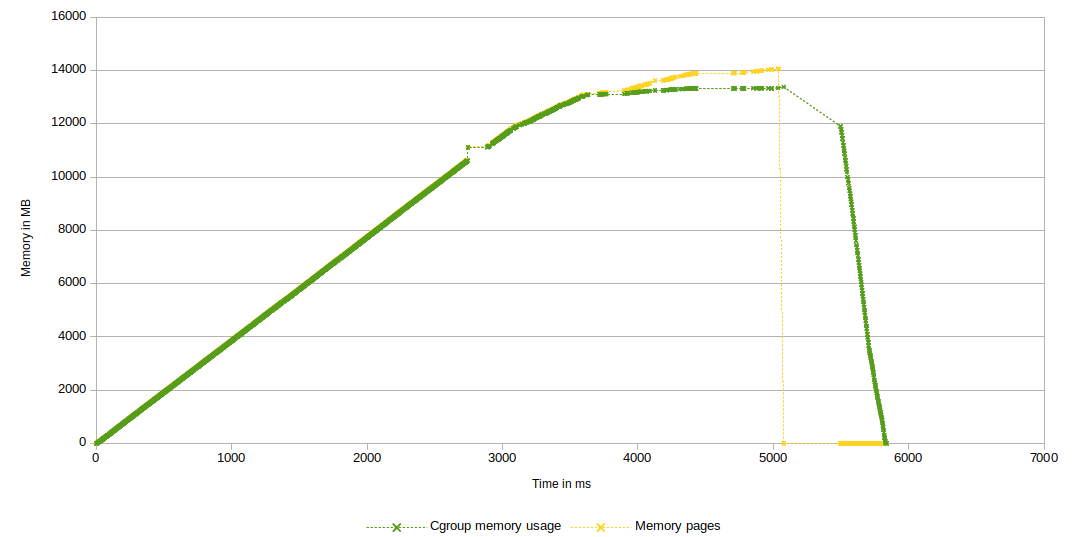
\includegraphics[width=1\linewidth]{pics/001,5_mem_usage_No_Limit_Cgroup_Pages_RDY_FOR_USE.png}
	\captionof{figure}[Speicher Verbrauch Cgroup 8200MB Limit]{Memory usage Cgroup 8200MB Limit}
	\label{fig:001,5_mem_usage_No_Limit_Cgroup_Pages_RDY_FOR_USE.png}
\end{minipage}

\subparagraph{Ergebnis Test03,5}
In Abbildung \ref{fig:001,5_mem_usage_No_Limit_Cgroup_Pages_RDY_FOR_USE.png} sind die 2GB Unterschied zwischen \emph{Cgroup memory usage} und den \emph{Memory Pages} offensichtlich nicht erreicht worden, was mehrere Gründe haben kann. Möglich ist eine zusätzliche Speicheranforderung des Betriebssystems, während der Prozess in der Paging-Phase war und zum früheren Absturz geführt hat. Auf den Effekt wird im Rahmen dieser Arbeit nicht genauer eingegangen.



\subparagraph{Test04}
In einem weiteren Schritt wird nun ein Container erstellt, der für eine gewisse Zeitspanne läuft. Das in Listing \ref{01mem} gezeigte Programm wird so modifiziert, dass das gesetzte Limit knapp überschritten wird und ist in Listing \ref{02mem} zu sehen. 

\vspace{1em}
\lstinputlisting[caption=einfacher C-Code, label=02mem, basicstyle=\ttfamily\scriptsize]{code/02mem.txt}

\subparagraph{Erwartungshaltung Test 04}
Nachdem der Malloc() Befehl jetzt 2200000-mal ausgeführt wird, sollte der Speicherverbrauch der Memory Pages nicht über 8600MB steigen und 60 Sekunden diesen Wert halten.



\[\mathrm{sizeof(int)} = 4 \mathrm{Byte}\]

\[\mathrm{sizeof(int)} * 1024 = 4 \mathrm{KB}\]

\[\mathrm{sizeof(int)} * 1024 * 2200000 \approx 8600 \mathrm{MB}\]


\vspace{1em}
\begin{minipage}{\linewidth}
	\centering
	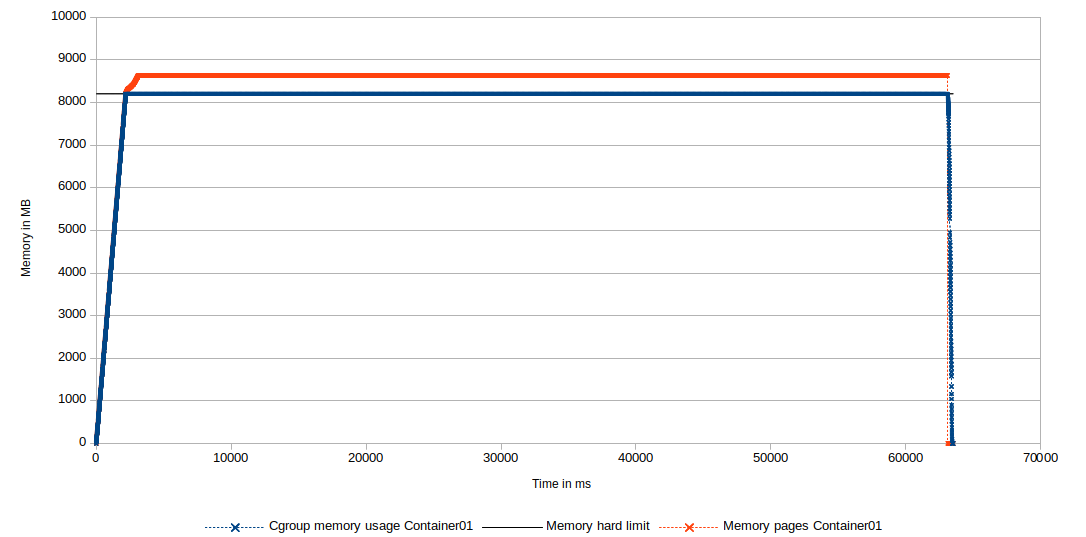
\includegraphics[width=1\linewidth]{pics/004_mem_usage_8200mb_limit_Container01_Basis_RDY_FOR_USE.png}
	\captionof{figure}[Speicher Verbrauch Cgroup 8200MB Limit]{Memory usage Cgroup 8200MB Limit}
	\label{fig:004_mem_usage_8200mb_limit_Container01_Basis_RDY_FOR_USE}
\end{minipage}

\subparagraph{Ergebnis Test04}
Wie in Abbildung \ref{fig:004_mem_usage_8200mb_limit_Container01_Basis_RDY_FOR_USE} zu entnehmen, ist es möglich für einen längeren Zeitraum über das Limit hinaus Ressourcen zu allokieren. Durch die lange Ausführungszeit gleichbleibender Ressourcen ist es jetzt möglich, den Einfluss von Containern untereinander zu untersuchen. Dieser Container wird von nun an als Container01 bezeichnet.

\subparagraph{Test05}
Im Ablauf des folgenden Tests wird zuerst Container01 gestartet und während der Laufzeit wird Container02 ebenfalls eingeschaltet. Der Container02 wird zum besseren Verständnis in Abbildung \ref{fig:005_mem_usage_8200mb_limit_Container02_Basis_RDY_FOR_USE_FOCUS} nochmals in skalierter Umgebung dargestellt. 


\vspace{1em}
\begin{minipage}{\linewidth}
	\centering
	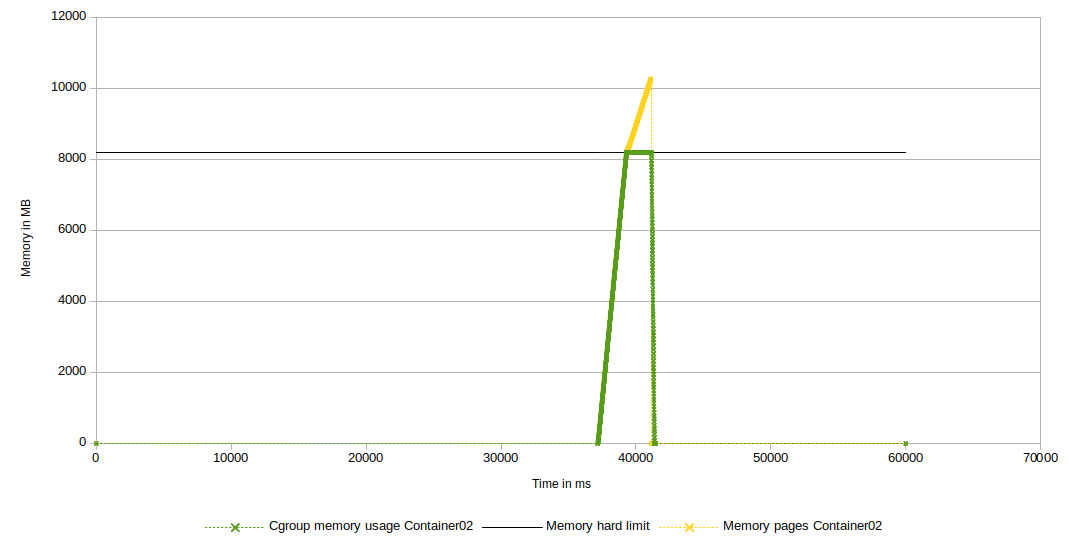
\includegraphics[width=1\linewidth]{pics/005_mem_usage_8200mb_limit_Container02_Basis_RDY_FOR_USE_FOCUS.png}
	\captionof{figure}[Speicher Verbrauch Cgroup 8200MB Limit]{Memory usage Cgroup 8200MB Limit}
	\label{fig:005_mem_usage_8200mb_limit_Container02_Basis_RDY_FOR_USE_FOCUS}
\end{minipage}

\subparagraph{Erwartungshaltung Test 05}
Die verwendbaren Systemressourcen liegen nach Abbildung \ref{fig:001_mem_usage_No_Limit_Cgroup_RDY_FOR_USE} bei etwa 14000MB. Allein Container01 verwendet schon ca. 8600MB der gesamten Summe, was die Deckelung von Container02 auf 8200MB rein rechnerisch unnötig macht. Somit wird Container02 frühzeitig beendet werden. 

\vspace{1em}
\begin{minipage}{\linewidth}
	\centering
	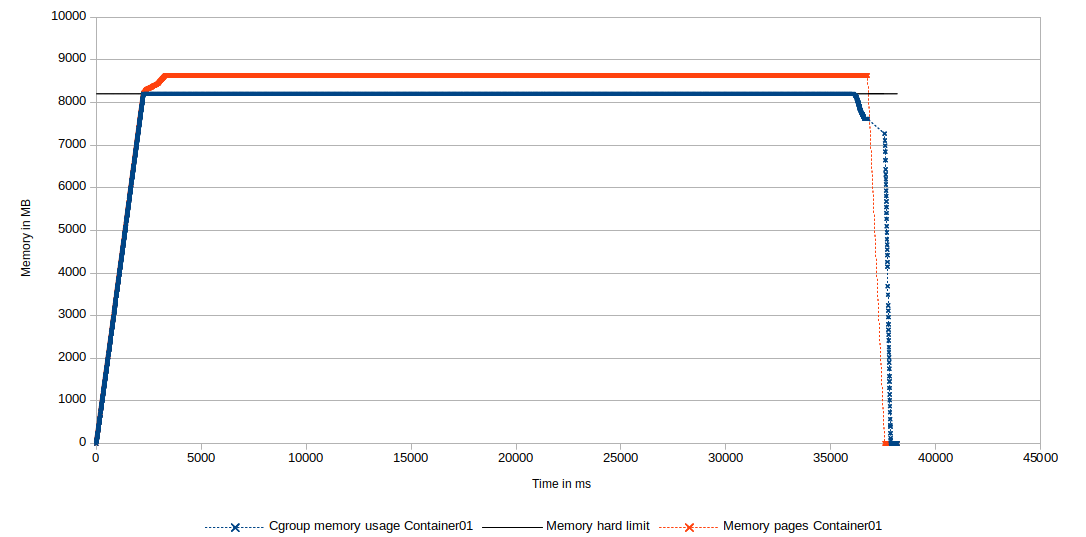
\includegraphics[width=1\linewidth]{pics/006_mem_usage_8200mb_limit_Container01_mit_ipact_RDY_FOR_USE.png}
	\captionof{figure}[Speicher Verbrauch Cgroup 8200MB Limit]{Memory usage Cgroup 8200MB Limit}
	\label{fig:006_mem_usage_8200mb_limit_Container01_mit_ipact_RDY_FOR_USE}
\end{minipage}

\subparagraph{Ergebnis Test05}
In Abbildung \ref{fig:006_mem_usage_8200mb_limit_Container01_mit_ipact_RDY_FOR_USE} ist zu erkennen, dass Container01 nicht nach ca. 63 Sekunden geplant beendet wurde, sondern schon etwa nach ca. 38 Sekunden.

Abbildung \ref{fig:007_mem_usage_8200mb_limit_Container01_und_Container02_RDY_FOR_USE} zeigt beide Container mit einer gemeinsamen Zeitachse. Nach dem Start von Container02, als dieser ca. 5100MB Speicher allokiert hat, wird Container01 beendet. Container02 überschreitet das Limit von 8200MB nach ca. 41 Sekunden und wird nach ca. 42,5 Sekunden ebenfalls beendet.

\vspace{1em}
\begin{minipage}{\linewidth}
	\centering
	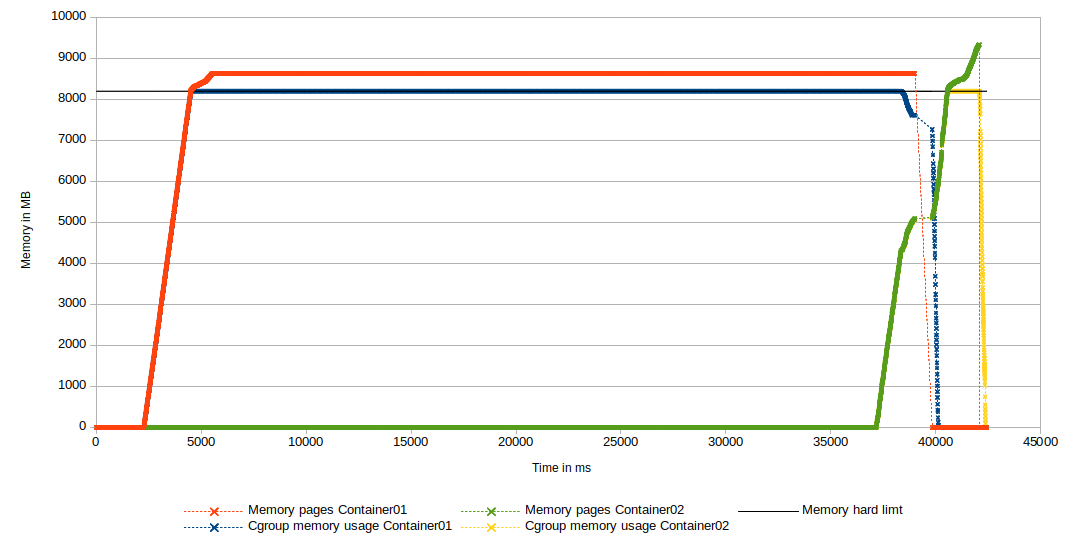
\includegraphics[width=1\linewidth]{pics/007_mem_usage_8200mb_limit_Container01_und_Container02_RDY_FOR_USE.png}
	\captionof{figure}[Speicher Verbrauch Cgroup 8200MB Limit]{Memory usage Cgroup 8200MB Limit}
	\label{fig:007_mem_usage_8200mb_limit_Container01_und_Container02_RDY_FOR_USE}
\end{minipage}

Der einzelne Verlauf der Graphen in Abbildung \ref{fig:008_mem_usage_8200mb_limit_Container01_und_Container02_RDY_FOR_USE_FOCUS} deutlicher zu sehen. Am auffälligsten ist die Lücke (mit gestrichelten Linien gekennzeichnet) in der Mitte der Abbildung. Eine Lücke entsteht, wenn über mehrere Millisekunden keine Messwerte vom Skript erfasst werden können. In diesem Fall ist das auf eine Systemüberlastung zurück zu führen, welche durch die Überlastung des Arbeitsspeichers und die dadurch eingeleiteten Systemreaktionen entstanden ist. 

\vspace{1em}
\begin{minipage}{\linewidth}
	\centering
	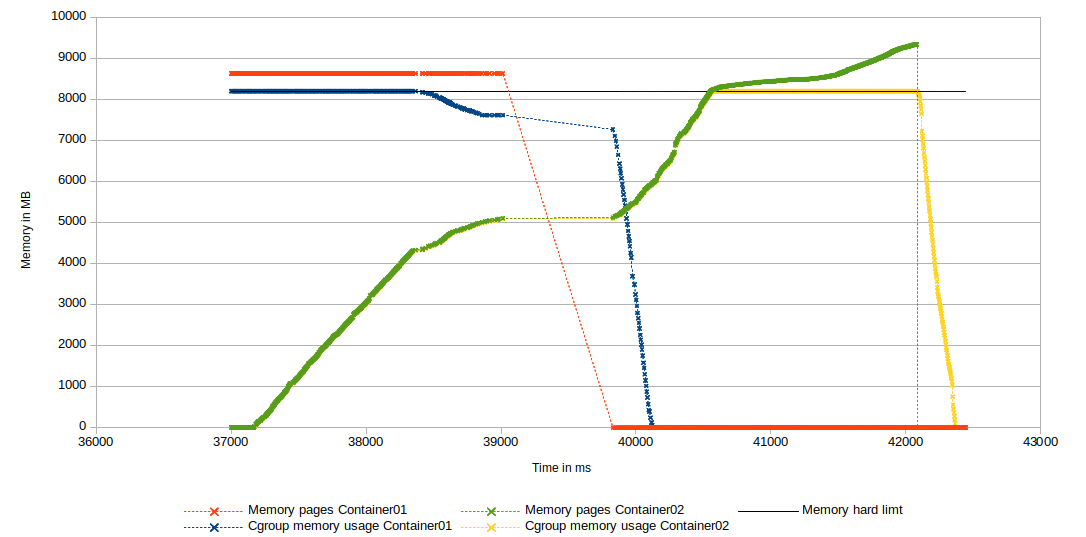
\includegraphics[width=1\linewidth]{pics/008_mem_usage_8200mb_limit_Container01_und_Container02_RDY_FOR_USE_FOCUS.png}
	\captionof{figure}[Speicher Verbrauch Cgroup 8200MB Limit]{Memory usage Cgroup 8200MB Limit}
	\label{fig:008_mem_usage_8200mb_limit_Container01_und_Container02_RDY_FOR_USE_FOCUS}
\end{minipage}



An der blauen Linie \emph{Cgroup memory usage Container01} in Abbildung \ref{fig:008_mem_usage_8200mb_limit_Container01_und_Container02_RDY_FOR_USE_FOCUS} ist nach ca. 38.5 Sekunden ein Abwärtstrend zu erkennen. Zu diesem Zeitpunkt hat das Betriebssystem mit dem Paging begonnen und lädt von der Cgroup allokierte Pages in den Massenspeicher. Die tatsächliche Menge an Arbeitsspeicher, welchen die Cgroup allokiert, nimmt ab. Die rote Linie \emph{Memory pages Container01} zeigt die Summe aller vom Prozess allokierten Memory Pages, folglich auch den auf den Massenspeicher ausgelagerten Anteil. Der Verlauf der grünen Linie \emph{Memory pages Container02} lässt sich durch folgende Annahme begründen. Wegen der erhöhten Anforderung an das I/O System was das Paging zu verantworten hat, verringert sich die Allokationsrate. Nach dem Beenden von Container01 wird ebenfalls das Paging beended. Dadurch verläuft die Steigung der Kurven von Container02 ähnlich wie nach dem Start des Prozesses. 

\subparagraph{Test06}
Bisher wurden Container betrachtet, die sich nicht an das vorgegebene Limit gehalten haben. Im Folgenden gilt es zu zeigen, dass auch bei \emph{gutartigen} Containern, also Container welche sich immer unter dem vorgegebenen Limit befinden, ähnliche Effekte auftreten. Für den folgenden Testdurchlauf wird der in Listing \ref{03mem} gezeigte C-Code verwendet. Zuerst startet Container03, der den eben genannten C-Code ausführt. Während des 60 Sekunden Sleep() startet Container04 ebenfalls mit dem in Container03 verwendeten Code.

\vspace{1em}
\lstinputlisting[caption=einfacher C-Code, label=03mem, basicstyle=\ttfamily\scriptsize]{code/03mem.txt}

\subparagraph{Erwartungshaltung Test 06}
Durch die Änderung auf 2048000 Wiederholungen des Malloc Befehls, wird Container03 bis ca. 8000MB Speicher allokieren. Nach dem Start von Container04 wird ein ähnlicher Graphenverlauf erwartet wie im vorherigen Test. Da das gesetzte Hard Limit bei 8200MB nicht überschritten wird, sollten die Linien \emph{Cgroup memory usage Container04} und \emph{Memory Pages Container04} identisch über die Lebensdauer des Containers verlaufen.

\vspace{1em}
\begin{minipage}{\linewidth}
	\centering
	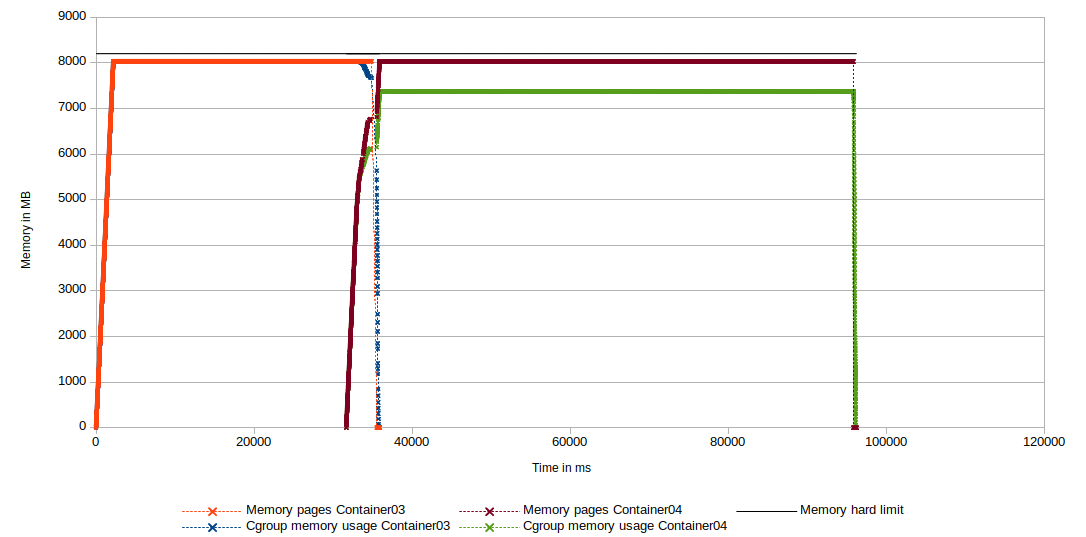
\includegraphics[width=1\linewidth]{pics/009_mem_usage_8200mb_limit_Container03_undContainer04_RDY_FOR_USE.png}
	\captionof{figure}[Speicher Verbrauch Cgroup 8200MB Limit]{Memory usage Cgroup 8200MB Limit}
	\label{fig:009_mem_usage_8200mb_limit_Container03_undContainer04_RDY_FOR_USE}
\end{minipage}

\subparagraph{Ergebnis Test06}
Der Verlauf von Container03 in Abbildung \ref{fig:009_mem_usage_8200mb_limit_Container03_undContainer04_RDY_FOR_USE} war Container01 in Abbildung \ref{fig:007_mem_usage_8200mb_limit_Container01_und_Container02_RDY_FOR_USE} sehr ähnlich. Betrachtet man in Abbildung \ref{fig:010_mem_usage_8200mb_limit_Container03_undContainer04_RDY_FOR_USE_Focu} die blaue Linie \emph{Cgroup memory usage Container03} und die dunkelrote Linie \emph{Cgroup memory usage Container04} fällt auf, dass das Betriebssystem nach ca. 33,5 Sekunden mit dem Paging angefangen hat und Einfluss auf die Cgroup beider Container nimmt. Das Resultat ist vergleichbar mit dem aus Abbildung \ref{fig:008_mem_usage_8200mb_limit_Container01_und_Container02_RDY_FOR_USE_FOCUS}.  

\vspace{1em}
\begin{minipage}{\linewidth}
	\centering
	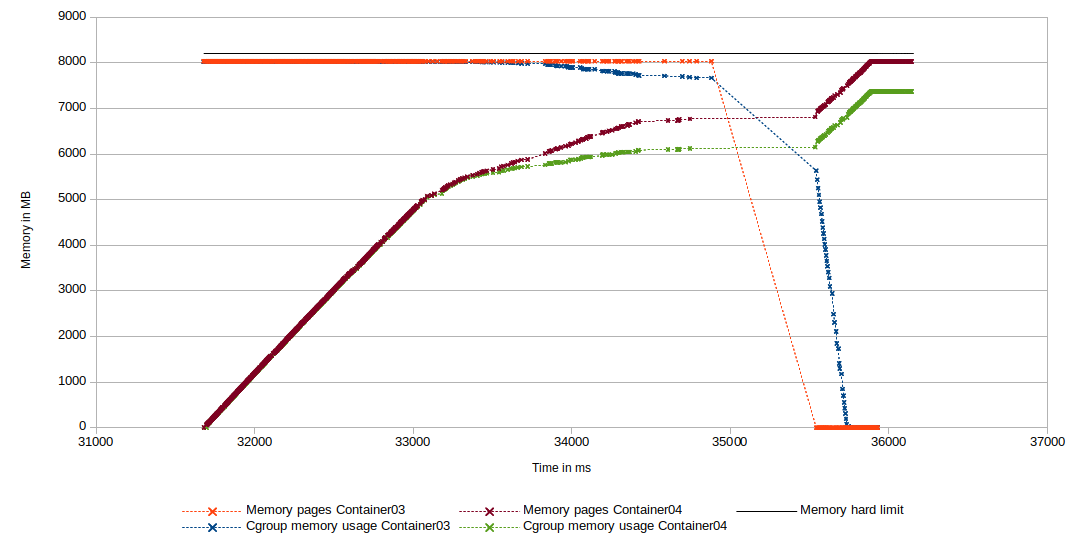
\includegraphics[width=1\linewidth]{pics/010_mem_usage_8200mb_limit_Container03_undContainer04_RDY_FOR_USE_Focus.png}
	\captionof{figure}[Speicher Verbrauch Cgroup 8200MB Limit]{Memory usage Cgroup 8200MB Limit}
	\label{fig:010_mem_usage_8200mb_limit_Container03_undContainer04_RDY_FOR_USE_Focu}
\end{minipage}

Container04 verläuft bei der Allokation unter dem gesetzten Limit wegen des Unterschiedes von der in Abbildung \ref{fig:009_mem_usage_8200mb_limit_Container03_undContainer04_RDY_FOR_USE} grün dargestellte Linie \emph{Cgroup memory usage Container04} und der dunkelroten Linie \emph{Memory pages Container04} nicht wie erwartet. In Abbildung\ref{fig:007_mem_usage_8200mb_limit_Container01_und_Container02_RDY_FOR_USE}war vor der Lücke nur die blau dargestellte Linie \emph{Cgroup memory usage Container01} vom Paging betroffen und die parallel zur grün verlaufende gelbe Linie \emph{Cgroup memory usage Container02} zeigte keine Anzeichen von Paging. Auch an dieser Stelle wird auf den Seiteffekt, verursacht durch das Paging nicht weiter eingegangen.

Es wurde gezeigt, dass ein neu ausgeführter Container mit den im Linux-Kernel implementierten Mechanismen in der Lage ist, einen bereits bestehenden Container zu beenden und dann auf dessen Ressourcen zuzugreifen.



\pagebreak
